\section{Surface Reconstructions}
The role of surface reconstructions in epitaxial crystal growth offers a rich field of future research. Both reconstructions involving steps and the atomic reconstructions of surfaces offer routes to driving epitaxial growth into new regimes not previously observed.
\subsection{Twinning Control}
In this work, offcut substrates and the surface reconstructions induced by them were demonstrated to be effective at suppressing the twinning common in face centered cubic semiconductors. These offcut substrates were all offcut toward the (110) direction, resulting in reconstructions and steps along a perpendicular (110) direction, leaving long terraces. Such stepping was successful at suppression twinning along that direction, but had no impact in the perpendicular direction. If instead the substrate is offcut towards a (100) direction, when reconstructed the resulting terraces will have step edges towards to perpendicular \{110\} directions. Such a reconstructed surface may be able to suppress twinning in both directions, resulting in overall a higher quality epitaxial growth.
\subsection{Lattice Matched Growth on Reconstructions}
This work showed that the locked-in high temperature reconstruction of a crystalline oxide could successfully support alignment of an epitaxial crystal of orientation different than that of the bulk crystalline substrate. While in this case the epitaxial growth was not substantially improved, there are a huge variety of stable surface reconstructions reported in the literature. These surface reconstructions may offer lattice matches to epitaxial crystals, allowing high quality growth were no bulk crystalline substrate exists.

Undergoing such a research project would require a survey of existing literature of surface reconstructions. Many publications do not provide the exact lattice spacings of atoms of the surface reconstruction. Participation of researchers which can successfully measure surface reconstructions would be essential to construction an extensive database. Once such a database were developed the lattice spacings of such reconstructions could be compared to existing epitaxial thin films and candidate pairs could be investigated by a variety of growth techniques.

The benefits of such systems would be the leveraging of existing substrates for the production of new epitaxial crystals.

\section{Epitaxial Liftoff}
The epitaxial liftoff process of CdTe/Al$_2$O$_3$ is a very surprising result considering the single crystal nature of film. There are a number of other materials which offer comparable lattice matches to either sapphire or another complex crystalline oxide. If these systems also exhibit the liftoff phenomenon the physics involved in such a process become even more interesting, and their engineering applications could allow previously expensive materials to be used in many systems. A patent application regarding the generalized liftoff process of crystalline materials on oxide substrates has been submitted and is being evaluated by the USPO.

\subsection{Other II-VI Liftoff}
Building on the prior successes of liftoff of CdTe on Sapphire it is expected that systems in the same chemical family may also exhibit the liftoff phenomenon. Based on these expectations, some preliminary experiemnts have been performed on CdTe grown on MgO and ZnTe grown on Sapphire. While CdTe/MgO does not result in a particularly high quality film due to the high chemical symmetry of the MgO surface, CdTe was found to a similar extent when grown on MgO. Similarly, as part of the continued investigation into II-VI systems, ZnTe/Al$_2$O$_3$ can be grown single phase with reasonable quality and also exhibits liftoff.
\begin{figure}
    \centering
    \begin{subfigure}[t]{0.5\textwidth}
        \centering
        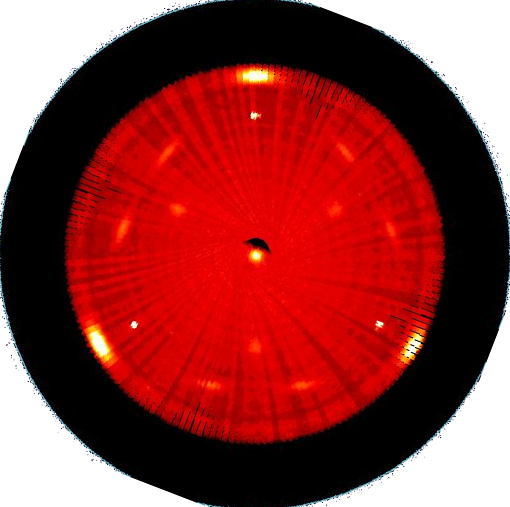
\includegraphics[width=0.97\textwidth]{znte_attached}
        \caption{\label{fig:znte_attached}ZnTe epitaxially grown on sapphire}
    \end{subfigure}%
    \begin{subfigure}[t]{0.5\textwidth}
        \centering
        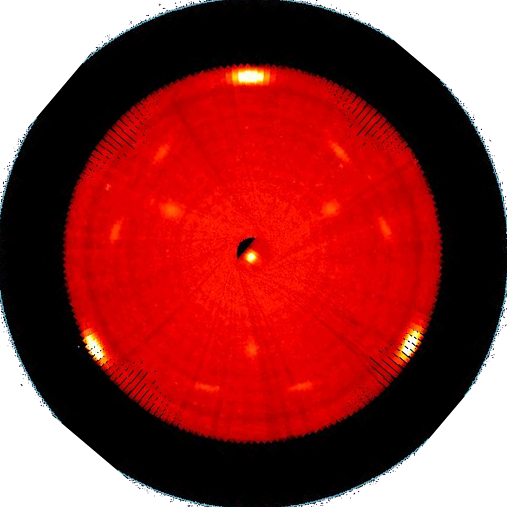
\includegraphics[width=0.97\textwidth]{znte_released}
        \caption{\label{fig:znte_released}ZnTe after liftoff on polysulphone carrier}
    \end{subfigure}
    \caption{\label{fig:znte_liftoff}Pre- and post-liftoff ZnTe}
\end{figure}

\subsection{III-V Liftoff}
There are several lattice matched or nearly lattice matched III-V material systems to single crystal oxide substrates. In many cases these systems have never had any attempts to grow epitaxial crystals. There is an expansive field of research open to investigate the growth of III-V materials on oxides.

One material system which was readily available for cursory experiments was InSb/Al$_2$O$_3$ which has a very similar lattice match to sapphire as CdTe. Initial investigations into InSb growth via MBE yielded films with twin volumes of $\sim$25\% comparable to poor CdTe grows. InSb/Al$_2$O$_3$ was also found to express the liftoff phenomenon.

The success of multiple substrate structures as well as the successes of both II-VI and III-V films indicates a number of other systems may also exhibit liftoff. The oxide substrates YAG, PbWO$_4$, GGG and YSZ offer suitable lattice matches to attempt single crystal growth which may then facilitiate liftoff. A full list of potential Semiconductor/Oxide lattice matches for liftoff will be presented in \cref{apndx:lattice-matches}.

\subsection{Physics of Liftoff}
The wide range of materials which are expected to demonstrate liftoff provides a rich research space to investigate the physics of liftoff. Immediate investigations into epitaxial process can be undertaken using density functional theory to investigate the energy landscape of the individual material systems at minimal cost. Interface sensitive in-situ growth characterization tools may provide some insight into the initial nucleation of layers during growth. Other buried interface techniques will need to be used to gain further insight into the liftoff process. The reverse process of attempting to grow an oxide on a semiconductor crystal may also provide some insight into the physics of liftoff.

\subsection{Engineering of Liftoff}
The liftoff processes performed thus far have used adhesive tapes or polymer carriers, investigating the simplicity of the liftoff process itself and the properties of the resulting films. Besides examining physics of the process and  expanding the material systems which have been demonstrated, there are a number of questions of engineering and application that could be explored.

Optimization of liftoff yield while still allowing for further processing is a delicate balance of strong and rigid carriers which are also potentially removable. Some of these are currently being investigated (polymers, wafer bonding) while there are others which have yet to be (vacuum, metal foils). Integration into electronic systems may require patterning or lithographic steps, the impact of such lithography on liftoff will also need to be investigated.

\section{Gold on Spinel}
The initial investigation of gold on spinel relied upon the discovery of a reproducible formation process and the measurement and modelling of the nanostructure formation process. The exact role of thickness, temperature, heating and cooling rate, and time spent at temperature were not investigated. A thorough investigation of such parameters has the potential to improve the formation density, uniformity and size. Control of such parameters is essential if such nanostructures are to be used in applications.

Some investigations into the formation of these nanostructures have found that the formation process is much richer than initial models investigations suggested. The spinel substrate, originally thought to be stable and static, appears to undergo significant solid state diffusion under the influence of gold. The substrate material appears to compose a significant portion of the intricate nanostructure. Work preformed by Tahereh Majdi has expanded the effective processing range and provided extensive TEM characterization\cite{tara-thesis}.